\documentclass[10pt, a4paper, oneside]{article}
\usepackage[english]{babel}
\usepackage{ragged2e}
\usepackage[nottoc]{tocbibind}
\usepackage{indentfirst}
\usepackage{graphicx}
\usepackage{hyperref}
\hypersetup{
    colorlinks=true,
    linkcolor=blue,
    filecolor=magenta,      
    urlcolor=cyan,
}

\urlstyle{same}
\graphicspath{ {/Users/yujiashi/Documents/IndependentStudy/RNA-seq_deconvolution_project/Report/
} }
% \setlength{\parindent}{2em} 
% \usepackage{hyperref}

\setlength{\parindent}{0pt}
\newcommand{\forceindent}{\leavevmode{\parindent=1em\indent}}
\title{RNA-seq Deconvolution Project Report}
\author{Yujia Shi}
\date{\today}

\begin{document}
\maketitle

\tableofcontents %—— 制作目录(目录是根据标题自动生成的)
\section{Introduction}
With the rapid development of single cell RNA-seq technologies, people can easily identify the precise cell-type specific expression
profile, which supports the research on cellular heterogenity. However, single cell RNA-seq technologies has not yet been widely
used due to its high cost and complicated experiment procedure. Given the advantages of cost and technical simplicity, bulk RNA-seq
is still the mainstream today. However, the existence of the cell-type specific single-cell expression profile allows us to extract the latent
information within bulk RNA-seq, such as the cell type composition. In this project, we explore the performance of weighted least square and iteratively reweighted
least square in the bulk RNA-seq deconvolution. We also benchmark our implementation with four mainstream deconvolution methods including deconRNASeq \cite{gong2013deconrnaseq}, Dtangle\cite{hunt2019dtangle} and
cibersort \cite{newman2015robust}.
\section{Method} %——一号子标题 

\subsection{Implementation} %——二号子标题  Beijing is the capital of China. 
\justify 
The IRLS method is implemented using Python 3.6. Source codes are available at \url{https://github.com/yujias424/RNA-seq_deconvolution_project}.

\subsection{Design of signature matrix and simulated bulk data}
\justify
To benchmark our approach with other methods using real dataset with non-simulated noise, 
we included multiple RNA-seq studies selected from metaSRA \cite{bernstein2017metasra}.
Total 263 studies and 4167 RNA-seq experiments were included in this analysis. 
The count table are normalized to count-per-million (CPM). 
We also pre-identified the cell type label of the experiment, and there are total 104 cell types. 

We propose that the systematic noise can be divided into two parts, including with-in study noise and cross-studies noise.
Due to the limitation of our data set, some cell types only have one corresponding study and thus 
the corss-studies variance is absent. To avoid the potential bias that some cell types may only have one type of systematic noise,
we exclude the cell type with less than two corresponding studies. There are 48 cell types left for further analysis.

In each simualted experiment, a noise-free signature matrix used for deonconvolution and a noisy signature matrix used for
generating the bulk data will be built. To generate the noisy signature matrix, we randomly select one experiment from a randomly picked
study for each cell type. The experiments from selected study will then excluded in the creation of noise-free siganture matrix.
For each cell type, the mean profile will be built using the rest of the experiments, which will be thus regarded as the 
signature profile of the corresponding cell type. The final noise-free cell-type signature matrix will be constructed by joining
aforementioned cell type specific mean profile.

The proposed proportion will be simulated using a dirichlet distribution, and the bulk data is generated by multiplying the
noisy signature matrix and the simulated proprotion.

\subsection{Marker genes selection}
\justify 
The marker genes will be selected using the similar approach described in Dtangle \cite{hunt2019dtangle}.
Dtangle will look at the ratio of the mean expression for each cell type to the sum of the mean expressions by all other cell types.
In our benchmark experiments, multiple thresholds are selected to determine the number of marker genes that are used for deconvolution.
The selection of quantile threshold will significantly effect the computational time.

\subsection{Weighted least square}
\justify
Our approach is developed based on the ordinary least squares approach \cite{gong2013deconrnaseq}. 
We first assume a noise-free RNA-seq data. The expression level of gene $i$ in such data
then can be modelled as following equation,
\begin{equation}
    y_{i} = \sum_{j=1}^N p_{j}x_{ij}
\end{equation}
where $p_{ij}$ denotes the proportion of cell type $j$ and $x_{ij}$ denotes the signature expression level of gene $i$ in cell type $j$.
In general, the equation can also be represented in matrix form as
\begin{equation}
    Y = \vec{P}X 
\end{equation}
where $Y$ is the bulk RNA-seq data to be deconvluted, $\vec{P}$ is the relative proportions of cell types and $X$ is the siganture matrix.

However, in real situation, the data we want to deconvolute often comes with heavy noise. The expression model in matrix form can then be modeled as
\begin{equation}
    Y = \vec{P}X + \epsilon
\end{equation}
where the $\epsilon$ is a noise term matrix contains the noise for all genes. The ordinary least squares approach assumes that
the noise of each genes is IID Gaussian white noise. In other words, the variance of the Gaussian distribution that different gene's noise
comes from is a constant. However, in real situation, the magnitude of different gene's noise is often not constant. For example, only the expression level of housekeeping genes included in some gene ontology groups
may hard to be effected by the disturbance of the experiment condition \cite{chen2014gene}. Therefore, the gene expression data 
in real situation can be often regarded as heteroskedastic data.

To solve the heteroskedastic data, we can apply the weighted least square approach, which aims at minimizing the weighted sum of squares rather than the residual sum of squares.
\begin{equation}
    WSS(X, \vec{P}) = \sum_{i=1}^N w_i(y_i - \vec{P} \cdot x_i)
\end{equation}
We still proposed that the each gene's noise term is a Gaussian, while their variance is not a constant. Assume that the noise
variance $\sigma_i^2$ of gene $i$ is known, we can give the gene $i$ a weight $1/\sigma_i^2$. The ordinary maximum likelihood estimate (MLE) then
can be turned to the heteroskedastic MLE, in which we can achieve a precise estimation on the proportion vector $\vec{P}$.

\subsection{Noise model}
\justify
As dicussed in weighted least square part, to achieve a proportion estimation with high accuracy, we need to have a through estimation
of the gene specific noise variance. In real situation, we can only observe the bulk data and the signature matrix. Therefore, it is 
natural for us to think about whether we can learn a function to describe the relationship between noise term variance $\sigma_i^2$ and the 
observed expression level $y_i$. 

To train a mean expression versus variance model, 
the variance for each gene will be firstly calculated by summing up the variance of gene in different cell types. 
We next built a mean profile based matrix consisting of 253 studies for 48 cell types as discussed in section 2.2, 
where each column represents the mean expression profile of a specific study containing the experiments labeled with the cell type. 
The model will then be trained using the gene's variance and corresponding mean expression level. 

\begin{figure}
    \centering
    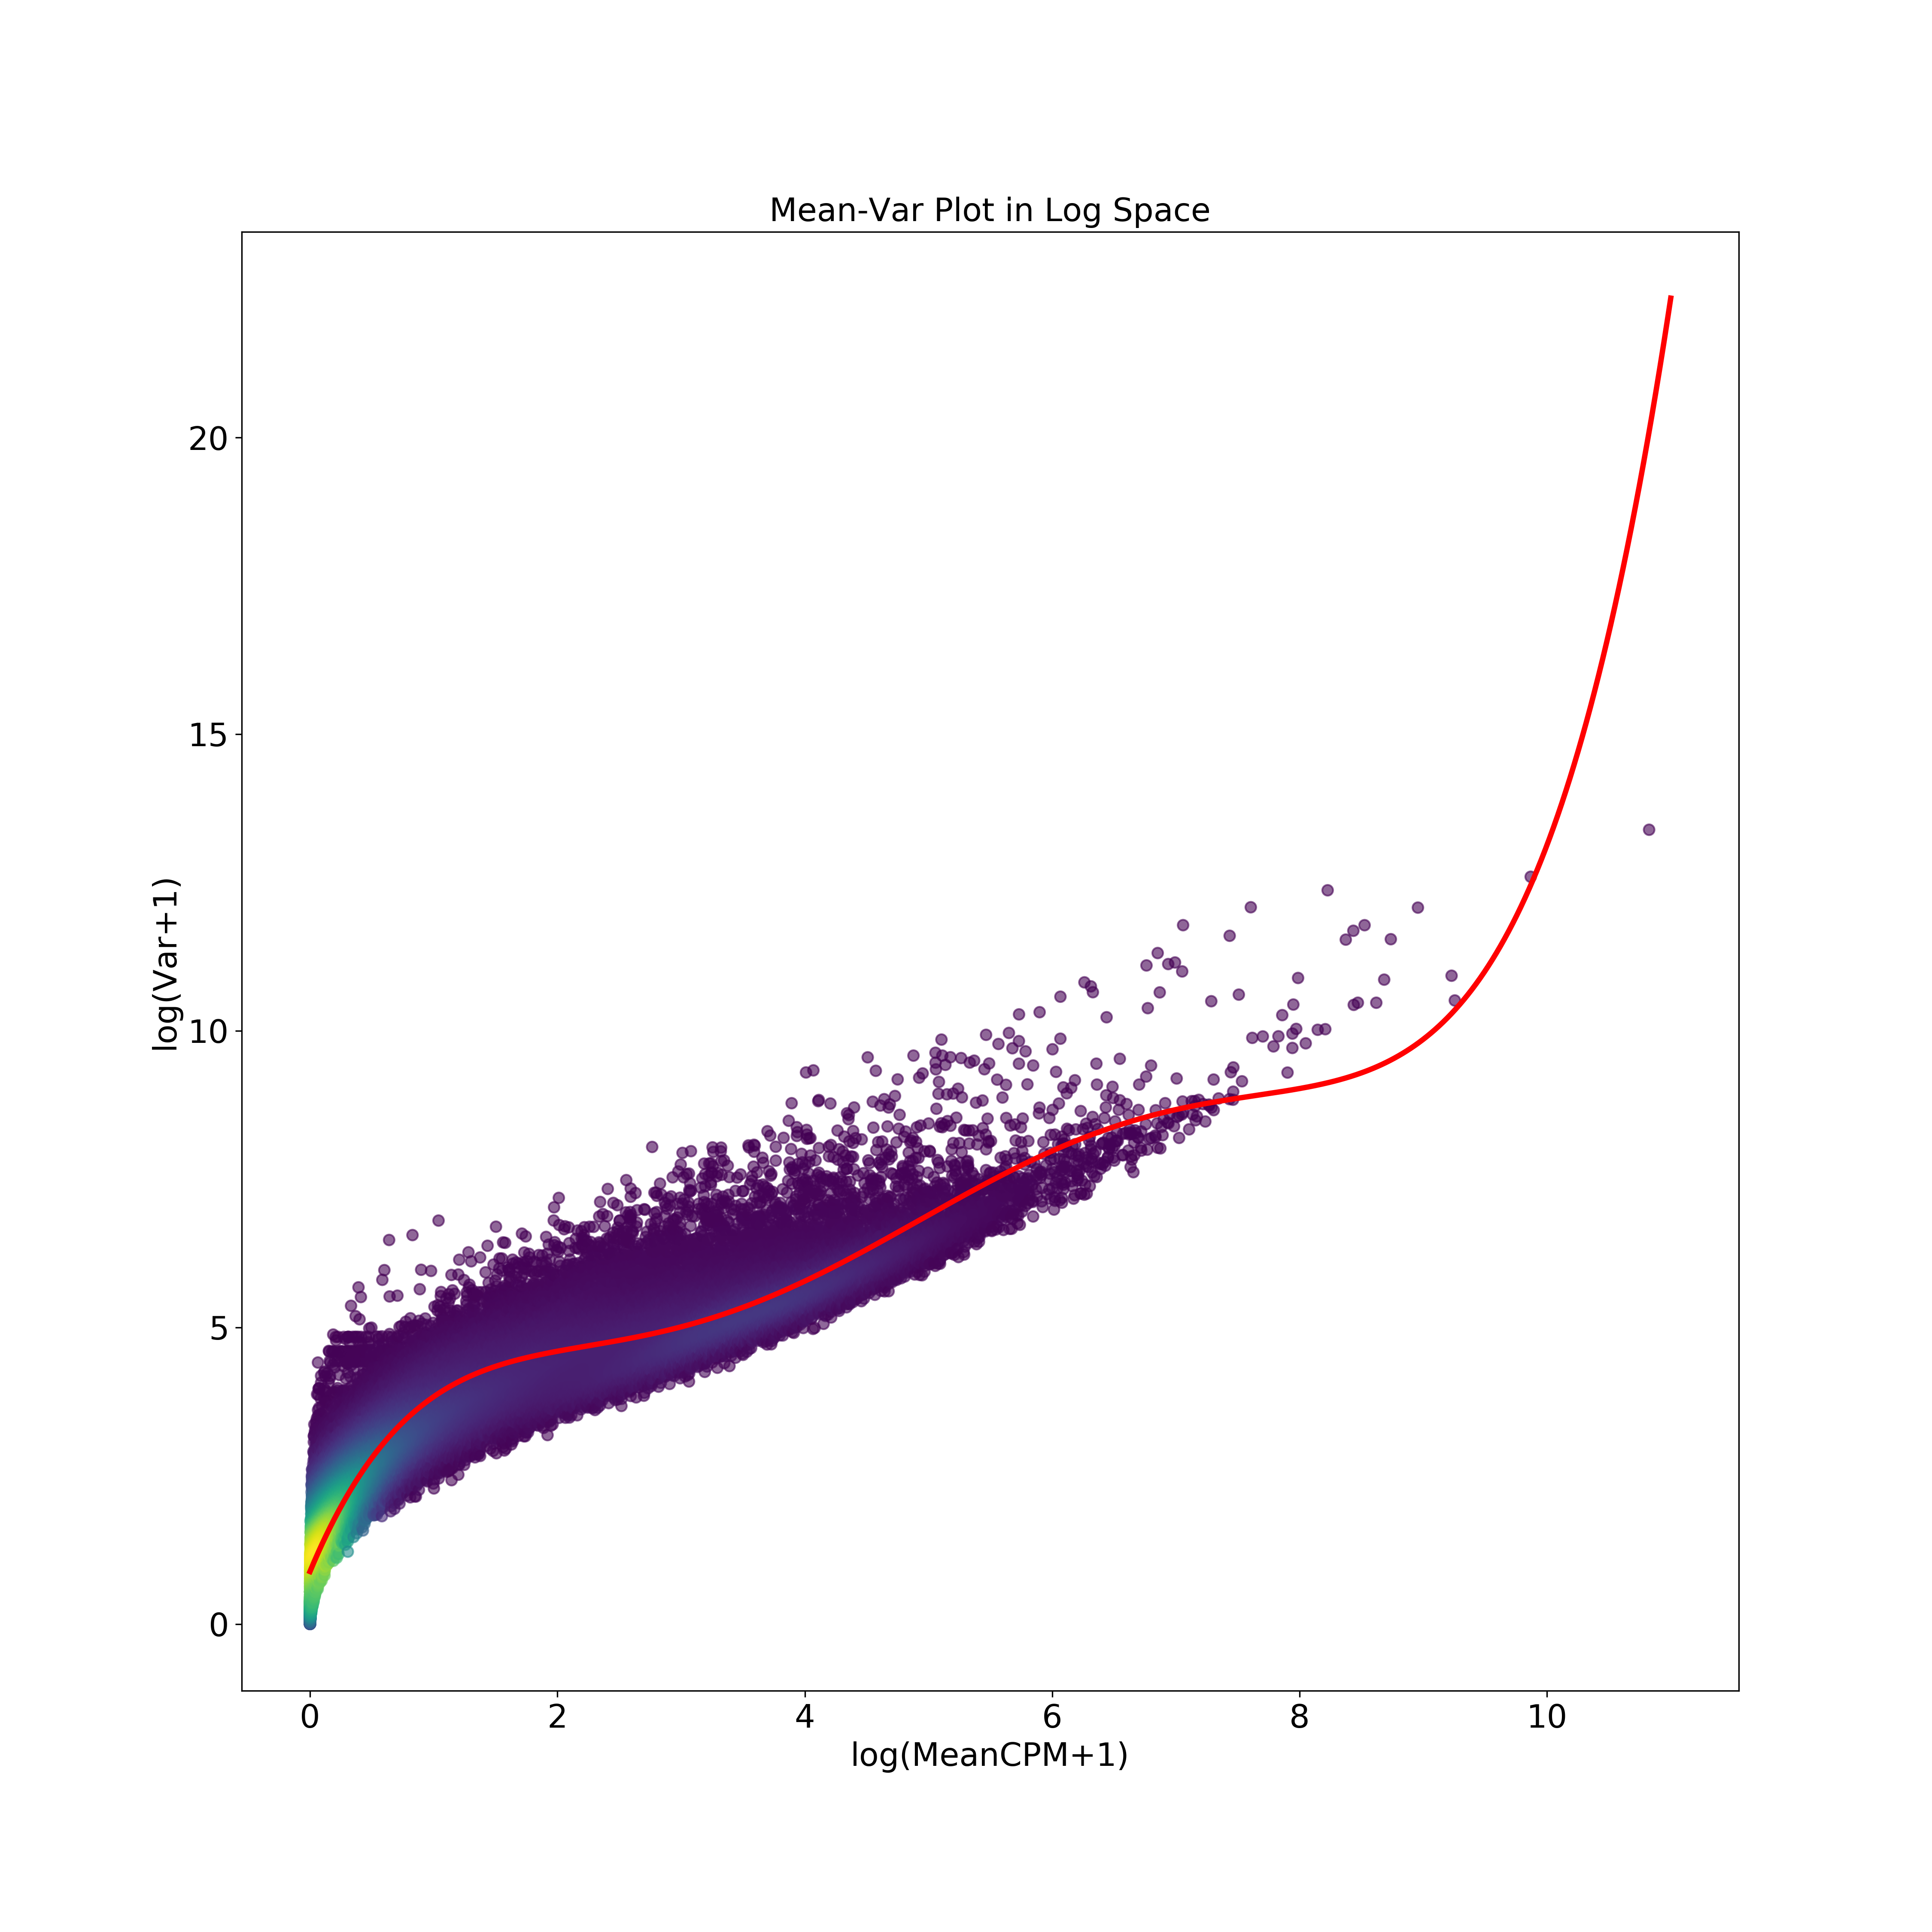
\includegraphics[width=8cm]{Var_Mean_model}
    \caption{Mean expression level versus Variance model in log space.}
    \label{fig1}
\end{figure}

Our model shows that the noise variance can be modeled by a function of experession level, which
can be directly as a tool to estimate the gene specific noise variance. Furthermore, we can notice that
the regression curve can be approximated as a linear function, indicating that it is possible for us
to directly use the expression level as the noise variance in practice.

\subsection{Creation of noise variance matrix}
\justify
Apart from estimating a function between noise term variance $\sigma_i^2$ and the observed expression level $y_i$, we may also propose that
the noise variance is independent with the observed expression level. Given a dataset with multiple studies and experiments used for constructing
the signature matrix, we can also learn a noise variance matrix withe the same shape as the signature matrix to describe the embedded noise of different
cell types.

We assume that different components of noise are independent Gaussian. Therefore, given the variance sum law, the variance of the cell-type specific noise can be calculated
through summing up all corresponding within studies variance and the cross studies variance. We can thus obtain the aforementioned variance matrix with same shape as
the signature matrix, which can be used for iteratively reweighted least square approach.

\subsection{Iteratively reweighted least square}
\justify
As the discussion about the variance model in the previous section, there are three types of the iteratively
reweighted least square (IRLS) approach. The difference between these three type of IRLS approach is that how these
method update the weights in each iteration.

The most simpliest approach is to use the observed expression level as an estimation of the noise variance.
Aforementioned variance model shows that the variance $\sigma_i^2$ can be approximately modeled as a linear function of the observed expression level. 
Therefore, the variance $\sigma_i^2$ can be directly replaced by the observed expression level. The weights are thus an identity function of
expression level. Inspired by the iteratively reweighted least squares, we can update the weights by multiplying the latest solution $\vec{P}^{(k)}$ and the signature matrix $X$.

Instead of using the idenity function of the expression level, we can also use the learned univariatespline function to get a more accurate estimation
of the noise variance (Figure \ref{fig1}). 

Last but not least, we can update the weights by multiplying the latest $\vec{P}$ and the learned variance matrix as well.
To be noticed, according to the variance sum law, we need to take a square of $\vec{P}$ before the multiply operation.
 
Convergence is reached when $||\vec{P}^{(k+1)} - \vec{P}^{(k)}|| \leq 0.01$.

\section{Results}  %——一号子标题 
\subsection{Learned model function based IRLS performs better than other mainstream methods}  %——二号子标题  Beijing is the capital of China.           
\justify
We benchmarked our implementation with other mainstrem methods. The L1-distance between estimated proportion and true proportion 
is used as the criterion to compare the
performance of different methods. We simulate the cell type composition using Dirichlet distribution with
four different parameter 0.001, 0.01, 0.1 and 1.
100 experiments were performed for each dirichlet parameter setting, and we compare the mean of the L1-distance results of these experiment
to identify the method with best performance. 

Figure 2 shows that the learned model based IRLS (IRLS\_lm) outperforms other approaches including deconRNASeq(NNLS), dtangle, cibersort and identity function based IRLS.
As expected, learned model will give a more accurate estimation of the noise variance and thus achieve a better performance compared with
the identity based IRLS. 

\subsection{Correct estimation of noise variance leads to a better result}
\justify
We may also want to see the performance of variance matrix based IRLS. Figure 3 shows that variance matrix based IRLS outperforms
other IRLS approaches. Studies used for creating the bulk data are also used for generating the variance matrix, meaning
that the variance matrix can capture the noise within the bulk data. This operation makes the variance matrix based IRLS obtain the 
best performance. However, in real situation, the siganture matrix is generated using the dataset which has no relationship with the bulk data to be deconvluted.
Therefore, afroementioned results indicates that the correct estimation of noise variance is a key step of the deconvolution algorithm.

\section{Discussion}
This project shows that the IRLS is a promising research direction of RNA-seq deconvolution. Our results indicates that a good estimation 
of gene-speicifc noise variance is an important compartment of the IRLS algorithm. Although the identity function based IRLS has a better computational time,
its performance cannot beat other IRLS approaches, meaning that expression level is an inaccurate estimation of the noise variance.

In the future, this project may focus on how to obstain an accurate estiamtion of the gene-specific noise variance from a given dataset.

\medskip

\bibliographystyle{unsrt}
\bibliography{citation}

\end{document}